\chapter{Introduction}

Current processors have multiple cores and their single core performance is improving only very slow because of physical limitations. On the other hand, the number of cores is still increasing and we can assume that this trend will continue. Therefore, development of parallel software is crucial for improvement of the overall performance.

Parallelization can be achieved manually or using some framework designed for it. For example, there are frameworks like OpenMP or Intel TBB. Department of Software Engineering at Charles University in Prague developed its own parallelization framework called Bobox\cite{bobox}.

Bobox is designed for parallel processing of large amounts of data. It was specifically created to simplify and speed up parallel programming of certain class of problems - data computations based on non-linear pipeline. It was successfully used in implementation of XQuery and TriQuery engines.

Bobox consists from runtime environment and operators. These operators are called boxes and they are C++ implementation of data processing algorithms. Boxes use messages called envelopes to send processed data to each other. 

Bobox takes as input execution plan written in special language Bobolang\cite{bobolang}. It allows to define used boxes and simply connect them into directed acyclic graph. Bobolang specifies the structure of whole application. It can create highly optimized evaluation, which is capable of using the most of the hardware resources.

Most used databases are relational. They are based on the view of data organized in tables called relations. An important language based on relational databases is Structured query language (SQL\cite{database}) which is used for querying data and  modifying content and structure of tables.

Architecture of planned SQL compiler is displayed in Figure~\ref{fig:sqlarchitecture}. 
\begin{figure}[h!]
  \centering

    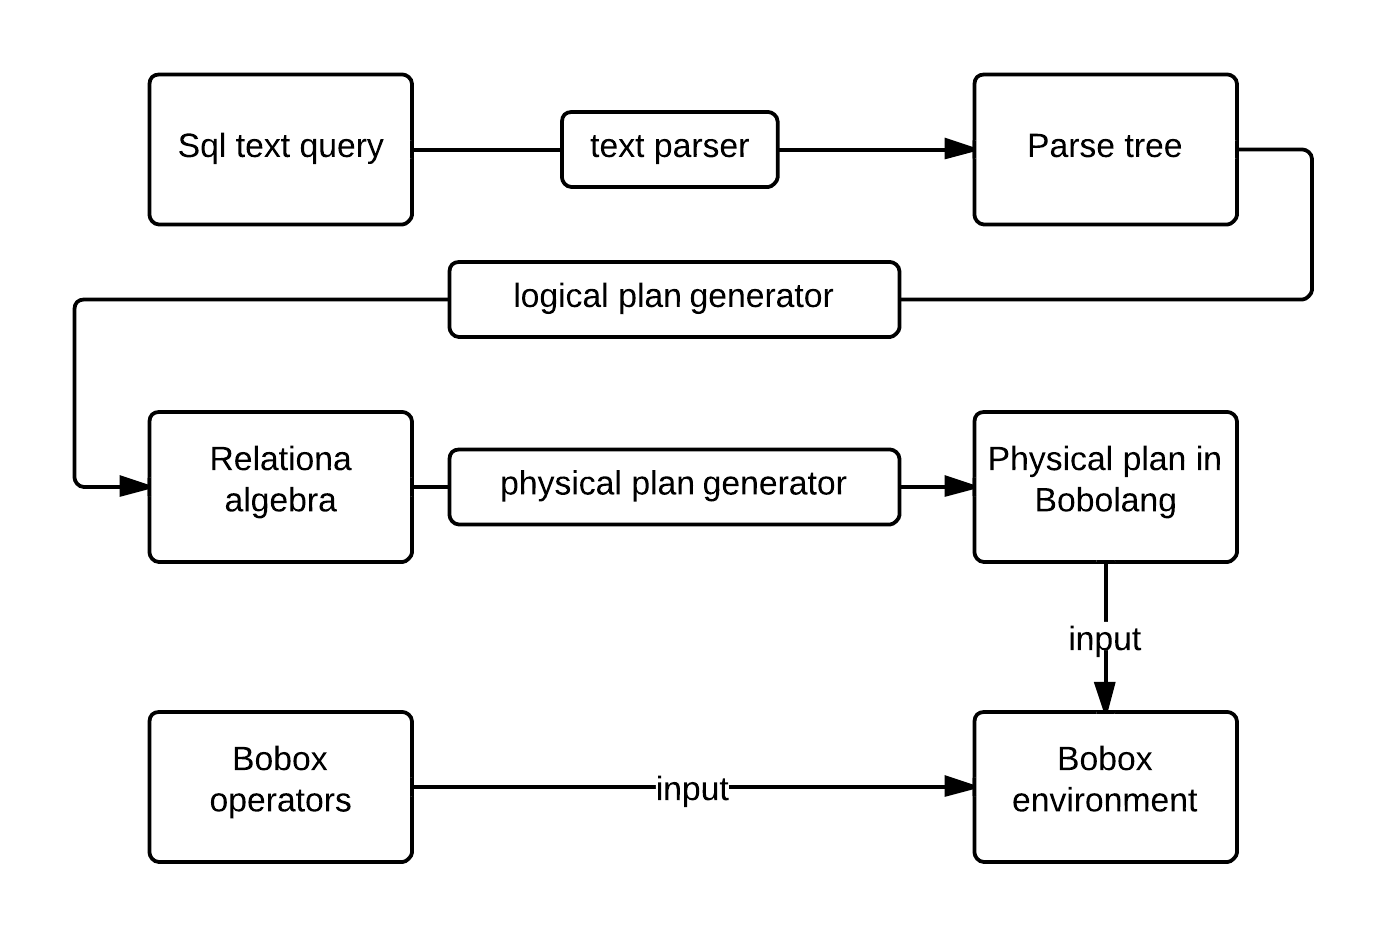
\includegraphics[width=1\textwidth]{sqlarchitecture}
    
      \caption{SQL compiler architecture.}
        \label{fig:sqlarchitecture}
\end{figure}
SQL query is written in text parsed into parse tree, which is transformed into logical query plan (Relational algebra). Relational algebra is then optimized and this form is used for generating physical query plan. Physical plan written in Bobolang is input for Bobox for execution. Besides physical plan, we need to provide implementation of physical algorithms (Bobox operators), as well.

Since SQL is a rather complicated language, the aim of this thesis is only implementing optimization and transformation of logical plan into physical plan. This part is displayed as physical plan generator in Figure~\ref{fig:sqlarchitecture}.


The main goal of this thesis is to implement part of SQL compiler. The input is a  query written in XML format in form of relational algebra. Program reads input and builds relational algebra tree, which is then checked for semantic errors. Then, we improve logical plan by pushing selection down the tree. We generate physical plan from improved relational algebra. In this phase, we assign physical algorithm for every logical plan operator and we also choose the order of joins. The output is an execution plan for Bobox written in Bobolang.
